\documentclass{article}
\usepackage[landscape]{geometry}
\usepackage{url}
\usepackage{multicol}
\usepackage{amsmath}
\usepackage{esint}
\usepackage{amsfonts}
\usepackage{tikz}
\usetikzlibrary{decorations.pathmorphing}
\usepackage{amsmath,amssymb}

\usepackage{colortbl}
\usepackage{xcolor}
\usepackage{mathtools}
\usepackage{amsmath,amssymb}
\usepackage{enumitem}
\usepackage{tcolorbox}
\makeatletter

\newcommand*\bigcdot{\mathpalette\bigcdot@{.5}}
\newcommand*\bigcdot@[2]{\mathbin{\vcenter{\hbox{\scalebox{#2}{$\m@th#1\bullet$}}}}}
\makeatother

\title{STAT 251 Formula Sheet}
%\usepackage[brazilian]{babel}
\usepackage[utf8]{inputenc}

\advance\topmargin-.8in
\advance\textheight3in
\advance\textwidth3in
\advance\oddsidemargin-1.45in
\advance\evensidemargin-1.45in
\parindent0pt
\parskip2pt
\newcommand{\hr}{\centerline{\rule{3.5in}{1pt}}}
%\colorbox[HTML]{e4e4e4}{\makebox[\textwidth-2\fboxsep][l]{texto}

\begin{document}

\begin{center}{\huge{\textbf{RECSYS Formula Sheet}}}\\
\end{center}
\begin{multicols*}{2}

\tikzstyle{mybox} = [draw=black, fill=white, very thick,
    rectangle, rounded corners, inner sep=5pt, inner ysep=10pt]
\tikzstyle{fancytitle} =[fill=black, text=white, font=\bfseries]
%% ---- 0. Global Effects ----
% --- Handy Theorems 
\begin{tikzpicture}
    \node [mybox] (box){%
        \begin{minipage}{0.48\textwidth}
        \begin{tabular}{lp{0.48\textwidth} l}
            1. Global Bias $\mu$ &
            $\mu = \frac{\sum_u \sum_{i}r_{ui}}{N + C}$

            $
                N = \# \text{non-zero ratings}
            $
            \\
            2. Normalization $r_{ui}'$ &
            $r_{ui}' = r_{ui} - \mu$
            \\
            3. Item Shrink Average Rating $b_i$ &
            $b_i = \frac{\sum_{u} r_{ui}'}{N_i + C}$

            $
                N_i = \text{number of Users who rated item } i
            $
            \\
            4. Normalization (Again) &
            $r_{ui}'' = r_{ui}' - b_i \ \forall u \in U, i \in I$    
            \\
            5. User Shrinked Average Rating $b_u$ &
            $b_u = \frac{\sum_{i \in I} r_{ui}''}{N_u}$
            \\
        \end{tabular}
        \begin{tcolorbox}[colback=gray!5, colframe=gray!80!black, title={Rating Estimation}]
            We can estimate a rating in a NON-PERSONALIZED way using the global effects:
            \begin{center}
                $r_{ui} = \mu + b_u + b_i$
            \end{center}
        \end{tcolorbox}
    \end{minipage}
};
%------------ Handy Theorems Header ---------------------
\node[fancytitle, right=10pt] at (box.north west) {Global Effects};
\end{tikzpicture}
%% ---- 1. Evaluation Techniques ----
% --- Evaluation Techniques ---
\begin{tikzpicture}
    \node [mybox] (box){%
        \begin{minipage}{0.48\textwidth}
        \begin{tabular}{lp{0.7\textwidth} l}
            \multicolumn{2}{l}{\textbf{Online Evaluation}} \\
            \hline
            Direct Feedback & User questionnaires (high bias) \\
            A/B Testing & Compare $RS_1$ vs $RS_2$ with unaware users \\
            Controlled Exp. & Small aware group, mock-up testing \\
            Crowdsourcing & Large volunteer group with compensation \\
            \hline
            \multicolumn{2}{l}{\textbf{Offline Evaluation}} \\
            \hline
            Tasks & Rating Prediction,Top-N \\
            Dataset Split & Training Set $\rightarrow$ Model Creation \\
            & User Profile $\rightarrow$ Rating Generation \\
            & Testing Set → Evaluation \\
            \hline
            \multicolumn{2}{l}{\textbf{Dataset Partitioning}} \\
            \hline
            Hold out of Ratings & Random \% of ratings for testing, Risk of overfitting \\
            Hold out of Users & Exclude users for training, Split excluded users' ratings between profile/testing \\
        \end{tabular}
        \end{minipage}
    };
\node[fancytitle, right=10pt] at (box.north west) {Evaluation Techniques};
\end{tikzpicture}
%% ---- 2. Classification Metrics ----
% Quality Metrics
\begin{tikzpicture}
    \node [mybox] (box){%
        \begin{minipage}{0.48\textwidth}
        \begin{tabular}{lp{0.8\textwidth} l}
            Metric & Description \\
            \hline
            Relevance & Ability of recommending items that the user likes \\
            Diversity & Ability of recommending different items \\
            Serendipity & Ability of recommending unexpected items \\
            Coverage & Ability of recommending items that the user has not seen \\
            Novelty & Ability of recommending unknown items \\
            Consistency & Ability to give consistent recommendations \\
            Confidence & Measure how much the model is sure about its recommendations \\
            Scalability & Time required for training \\
            Serving Time & Time required for serving recommendations \\
            Fairness & Fair recommendation for all users and for content providers \\
        \end{tabular}
        \end{minipage}
    };

% --- Quality Metrics header ---
\node[fancytitle, right=10pt] at (box.north west) {Quality Metrics};
\end{tikzpicture}

% --- Classification Metrics ---
\begin{tikzpicture}
    \node [mybox] (box){%
        \begin{minipage}{0.48\textwidth}
        \begin{center}
            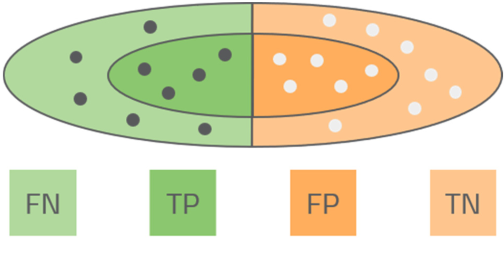
\includegraphics[height=0.1\textheight]{imgs/02_metrics.png}
        \end{center}
        \begin{tabular}{lp{0.8\textwidth} l}
            Classification Metrics & Formula \\
            \hline
            Recall & $\frac{TP}{FN + TP}$ 
            \\
            
            Precision & $\frac{TP}{TP + FP}$ 
            \\
            
            Fallout & $\frac{FP}{FP + TN}$ 
            \\
            Ranking Metrics & \\
            \hline
            AUC & $\frac{\sum_{k} Recall(k) \cdot \Delta Fallout}{N_i}$ 
            \\
            
            AP & $\sum_{k} Precision(k) \cdot [Recall(k) - Recall(k - 1)]$ 
            \\

            MAP & $\frac{\sum_u AP_u(k)}{N_u}$
        \end{tabular}
        \end{minipage}
    };

% --- Classification Metrics header ---

\node[fancytitle, right=10pt] at (box.north west) {Classification Metrics};

\end{tikzpicture}
%% ---- 3. Content-Based Filtering ----
% --- Content-Based Filtering ---
\begin{tikzpicture}
    \node [mybox] (box){%
        \begin{minipage}{0.48\textwidth}
        \begin{tabular}{lp{0.7\textwidth} l}
            \multicolumn{2}{l}{\textbf{Similarity Metrics}} \\
            \hline
            Basic Similarity & $s_{ij} = \vec{i} \cdot \vec{j}$ = \#common attributes \\
            Cosine Similarity & $s_{ij} = \frac{\vec{i} \cdot \vec{j}}{\|\vec{i}\| \cdot \|\vec{j}\|}$ \\
            Shrinked Cosine & $s_{ij} = \frac{\vec{i} \cdot \vec{j}}{\|\vec{i}\| \cdot \|\vec{j}\| + C}$ \\
            \hline
            \multicolumn{2}{l}{\textbf{Rating Estimation}} \\
            \hline
            Single Rating & $\tilde{r}_{ui} = \frac{\sum_{j} r_{uj} \cdot s_{ij}}{\sum_{j} s_{ij}}$ \\
            Matrix Form & $\tilde{R} = R \cdot S$ \\
            \hline
            \multicolumn{2}{l}{\textbf{k-Nearest Neighbors (kNN)}} \\
            \hline
            Definition & Keep only k highest similarity values per item \\
            Effect & Reduces noise and improves computation speed \\
            Selection & k too small: unreliable estimates \\
            & k too large: noisy recommendations \\
            Formula & $\tilde{r}_{ui} = \frac{\sum_{j, i \in N_k(j)} r_{uj} \cdot s_{ji}}{\sum_{j, i \in N_k(j)} s_{ji}}$ \\
            \hline
            \multicolumn{2}{l}{\textbf{TF-IDF Weighting}} \\
            \hline
            Term Frequency & $TF_{i,a} = \frac{N_{i,a}}{N_i}$ \\
            & $N_{i,a}$: occurrences of attribute $a$ in item $i$ \\
            & $N_i$: attributes in item $i$ \\
            \hline
            Inverse Doc Freq & $IDF_a = \log_2\frac{N_{items}}{N_a}$ \\
            & $N_{items}$: total items \\
            & $N_a$: items with attribute $a$ \\
        \end{tabular}
        \end{minipage}
    };
\node[fancytitle, right=10pt] at (box.north west) {Content-Based Filtering};
\end{tikzpicture}

%% ---- 4. Collaborative Filtering ----
% --- Collaborative Filtering ---
\begin{tikzpicture}
    \node [mybox] (box){%
        \begin{minipage}{0.48\textwidth}
        \textbf{User-based CF} aims to find similar users and recommend items based on their preferences.\par
        \begin{tabular}{lp{0.5\textwidth} l}
            Similarity & Formula & Context \\
            \hline
            Cosine Similarity & $s_{ij} = \frac{\vec{i} \cdot \vec{j}}{\|\vec{i}\| \cdot \|\vec{j}\|}$ & Implicit ratings \\
            Jaccard Similarity & $s_{ij} = \frac{\vec{i} \cap \vec{j}}{\vec{i} \cup \vec{j}}$ & Implicit ratings \\
            Pearson Correlation & 
            $s_{ij} = 
            \frac{
                \sum_{i \in I} 
                    (r_{iu} - \bar{r}_u) \cdot
                    (r_{iv} - \bar{r}_v)
                }
                {
                    \sqrt{\sum_{i \in I} (r_{iu} - \bar{r}_u)^2} 
                    \sqrt{\sum_{i \in I} (r_{iv} - \bar{r}_v)^2}
                }$ & Explicit ratings \\
        \end{tabular}
        \begin{tcolorbox}[colback=gray!5, colframe=gray!80!black, title={Focus on Pearson Correlation}]
            Pearson correlation computes similarity between a rating delta. Therefore the similarity is used to predict the delta of the rating!
            \\
            \begin{center}
            $\tilde{r}_{ui} - \bar{r}_u = 
               \frac{
                \sum{v \in KNN(u)}(r_{vi} - \bar{r}_{v})\cdot s_{uv}
               }
               {
                \sum{v \in KNN(u)} s_{uv}
               }
            $
            \end{center}
            

            
        \end{tcolorbox}

        \textbf{Item-based CF} aims to find similarity between items based how many users have the same opinion about them. The similarity is obtained in the same way as for user-based CF, considering the items instead of the users.\par

        \begin{tcolorbox}[colback=gray!5, colframe=gray!80!black, title={Memory-Based vs Model-Based}]
            \textbf{Memory-Based:}
            \begin{itemize}[label={--}, topsep=0cm, parsep=0cm, itemsep=0cm]
                \item Requires user profile in URM used to build model
                \item Only works for "known" users
                \item Must rebuild model for new users
                \item Example: User-Based CF (uses user neighborhood)
            \end{itemize}
            
            \textbf{Model-Based:}
            \begin{itemize}[label={--}, topsep=0cm, parsep=0cm, itemsep=0cm]
                \item Works with any user profile
                \item Supports both "known" and "unknown" users
                \item No model recomputation needed for new users
                \item Example: Item-Based CF (uses item similarities)
            \end{itemize}
        \end{tcolorbox}

        \begin{tcolorbox}[colback=gray!5, colframe=gray!80!black, title={Association Rules}]
            Association rules explore relationships between items using conditional probability:
            \begin{center}
            $P(i|j) = \frac{\text{\# appearances of i and j}}{\text{\# appearances of j} + C}$
            \end{center}
            where C is a shrinkage term to avoid biases. The similarity is asymmetric: $P(i|j) \neq P(j|i)$
        \end{tcolorbox}

        
        \end{minipage}
    };

% --- Collaborative Filtering header ---
\node[fancytitle, right=10pt] at (box.north west) {Collaborative Filtering};

\end{tikzpicture}
%% ---- 5. Machine Learning Item-based CF ----
% -- Machine Learning Item-based CF --
\begin{tikzpicture}
    \node [mybox] (box){%
        \begin{minipage}{0.48\textwidth}
            \begin{tabular}{lp{0.5\textwidth} l}
                % --- Formulas for Chapter A5: Item-Based CF with a Machine Learning Approach ---
                \textbf{Loss Functions} & 
                \\
                
                \hline
                
                Error Metrics & MAE,MSE
                \\
                Accuracy Metrics & Precision, Recall
                \\
                Ranking Metrics & AUC, MAP
                \\
                \hline
                \textbf{SLIM} (opt. Error Metric) & 
                \\

                \hline
                % Closed-Form Solution Objective
                Closed-Form Solution Objective &
                $
                S^* = \arg \min_S \left\| R - RS \right\|_2
                $
                \\
                % Constraint on Similarity Matrix Diagonal
                Constraints on S &
                $
                \text{diag}(S) = 0
                $
                \\

                    % Lasso Regression Regularization
                Lasso Regression Regularization &
                $
                S^* = \arg \min_S \left( \left\| R - RS \right\|_2 + \lambda \left\| S \right\|_1 \right)
                $
                \\
                % Ridge Regression Regularization
                Ridge Regression Regularization &
                $
                S^* = \arg \min_S \left( \left\| R - RS \right\|_2 + \lambda \left\| S \right\|_2 \right)
                $
                \\

                % Elastic Net Regularization
                Elastic Net Regularization &    
                $
                S^* = \arg \min_S \left( \left\| R - RS \right\|_2 + \lambda_1 \left\| S \right\|_1 + \lambda_2 \left\| S \right\|_2 \right)
                $
                \\

                \hline
                \textbf{BPR} (opt. Ranking)& 
                \\
                \hline
                % Bayesian Probabilistic Ranking (BPR) Probability Function
                (BPR) Probability Function &
                $
                P(\tilde{r}_{ui} > \tilde{r}_{uj} \mid \text{user } u) = \sigma(x) = \frac{1}{1 + e^{-x}}
                $
                \\

                % Pairwise Difference for BPR
                Pairwise Difference for BPR &
                $
                x_{uij} = \tilde{r}_{ui} - \tilde{r}_{uj}
                $
                \\

            \end{tabular}
            \begin{tcolorbox}[colback=gray!5, colframe=gray!80!black, title={BPR optimization}]
                It can be demonstrated that optimizing the BPR objective function is equivalent to maximizing the AUC metric.
                Thus, BPR is an optimization method for ranking metrics.
                \begin{center}
                    \begin{align}
                        P(\tilde{r}_{ui} > \tilde{r}_{uj} \mid \text{user } u) &= P(\tilde{r}_{ui} - \tilde{r}_{uj} > 0  \mid \text{user } u) \\
                        &= P(x_{uij} > 0 \mid \text{user } u) \\
                        &= \sigma(x_{uij}) = \frac{1}{1 + e^{-x_{uij}}}
                    \end{align}
                \end{center}
                Where $\sigma(x)$ is the sigmoid function to optimize.
                \begin{itemize}[label={--}, topsep=0cm, parsep=0cm, itemsep=0cm]
                    \item $x_{uij}$ should tend to 1 if i is a relevant item for user u and j is not
                    \item $x_{uij}$ should tend to 0 if both items are not relevant for user u or either both relevant
                \end{itemize}
            \end{tcolorbox}
        \end{minipage}
    };
% -- Machine Learning Item-based CF Header --
\node[fancytitle, right=10pt] at (box.north west) {Machine Learning Item-based CF};


\end{tikzpicture}



%% ---- 6. Matrix Factorization ----
% -- Matrix Factorization --
\begin{tikzpicture}
    \node [mybox] (box){%
        \begin{minipage}{0.48\textwidth}
            \begin{tabular}{lp{0.5\textwidth} l}
                % --- Formulas for Chapter A6: Matrix Factorization ---
                \textbf{User Rating Matrix (URM)} & 
                \\
                
                \hline
                
                User Preference & $x_{uk}$: Preference of user $u$ for feature $k$ 
                \\
                Item Description & $y_{ik}$: Description of item $i$ for feature $k$
                \\
                Predicted Rating & $\tilde{r}_{ui} = \sum_k x_{uk} \cdot y_{ik}$ 
                \\
                Dimensionality Constraint & $ N_k < \frac{N_u \cdot N_i}{N_u + N_i} $
                \\

                \hline
                % Matrix Product
                Matrix Factorization & 
                $R \approx X \cdot Y$ 
                \\
                % Dimensions
                Dimensions & $X \in \mathbb{R}^{N_u \times N_f}, Y \in \mathbb{R}^{N_f \times N_i}, R \in \mathbb{R}^{N_u \times N_i}$
                \\

                \hline
                % Loss Function
                Loss Function & 
                $\min_{X, Y} \| R - XY \|_2$
                \\
                % Regularization
                Regularization & 
                $
                \min_{X, Y} \| R - XY \|_2 
                + \lambda_1 \|X\|_2 + \lambda_2 \|Y\|_2
                $
                \\
                \hline
                % SGD for MF
                SGD for MF & 
                \begin{minipage}{0.5\textwidth}
                    - Sample $(u, i, r_{ui})$
                    \\
                    - $\frac{\delta E(X,Y)}{\delta x_u} = 
                    - 2 \cdot (r_{ui} - x_u y_{i*})  \cdot y_{i*}
                    + 2 \lambda_1 \cdot x_u$
                    \\
                    - $\frac{\delta E(X,Y)}{\delta y_{i*}} = 
                    - 2 \cdot (r_{ui} - x_u y_{i*}) \cdot x_u
                    + 2 \lambda_2 \cdot y_{i*}$
                \end{minipage}
                \\
                \hline
                % Assumptions
                Missing Ratings & 
                \begin{itemize}[label={--}, topsep=0cm, parsep=0cm, itemsep=0cm]
                    \item[$\circ$] MAR: Missing As Random
                    \item[$\bullet$] MAN: Missing As Negative
                \end{itemize}
                \\  
                \hline
                \\

                % ALS alternative Least Squares Algorithm
                ALS Algorithm & 
                \begin{minipage}{0.5\textwidth}
                    \texttt{While not converged do:} \\
                    \quad \texttt{Fix $X$, Learn $Y$} \\
                    \quad \texttt{Fix $Y$, Learn $X$} \\
                \end{minipage}
                \\
                % FunkSVD Algorithm
                $\circ$ FunkSVD Algorithm & 
                \begin{minipage}{0.5\textwidth}
                    \texttt{set $N_k = 0$} \\
                    \texttt{Initialize $X, Y$} \\
                    \texttt{While not converged do:} \\
                    \quad \texttt{Increment $N_k$} \\
                    \quad \texttt{Apply ALS for current $N_k$} \\
                \end{minipage}
                \\
                \hline
                \\
                % SVD++
                SVD++ (train with SGD)& 
                \begin{minipage}{0.5\textwidth}
                    - $ \tilde{r}_{ui} = \mu + b_u + b_i + \sum_{k} x_{uk} \cdot y_{ki} $
                    \\
                    - $ \mu^*, b_u^*, b_i^*, X^*, Y^* = \min_{\mu, b_u, b_i, X, Y} E(\dots) $
                    
                \end{minipage}
                
                \\
                \hline
                \\
                % Asymmetric SVD
                Asymmetric SVD (m-b) & 
                $\tilde{R} = R Z Y \ , X = R Z$
                \\

                % Singular Value Decomposition
                $\bullet$ pure SVD (m-b) & 
                $\tilde{R} = U_k \Sigma_k V_k^T = R V_k V_k^T$
                \\

            \end{tabular}
        \end{minipage}
    };
% -- Matrix Factorization Header --
\node[fancytitle, right=10pt] at (box.north west) {Matrix Factorization};

\end{tikzpicture}

%% ---- 7. Hybrid Recommenders ----
% -- Hybrid Recommenders --
\begin{tikzpicture}
    \node [mybox] (box) {
        \begin{minipage}{0.48\textwidth}
            \begin{tabular}{lp{0.5\textwidth} l}
                Linear Combination & 
                \hfill 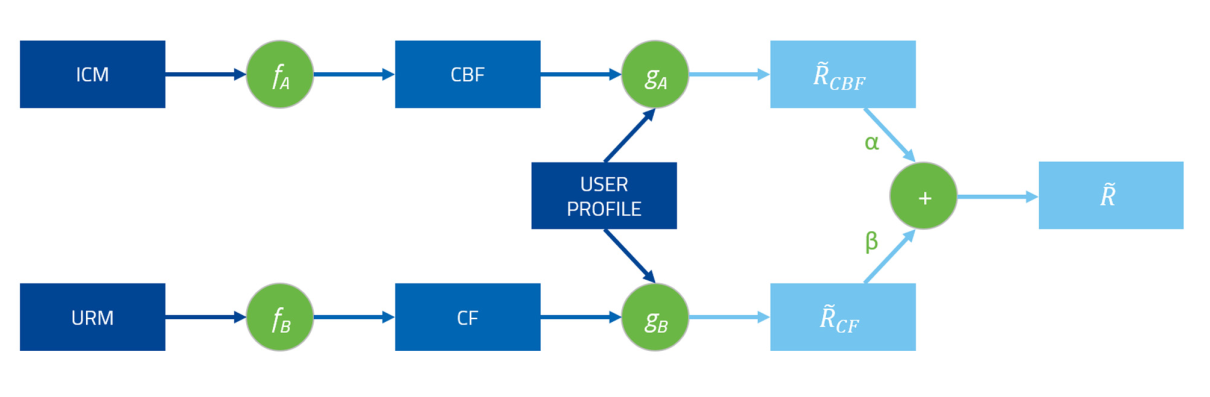
\includegraphics[width=0.35\textwidth]{imgs/071_LinearCombination.png}
                \\
                \hline
                List Combination & 
                \hfill 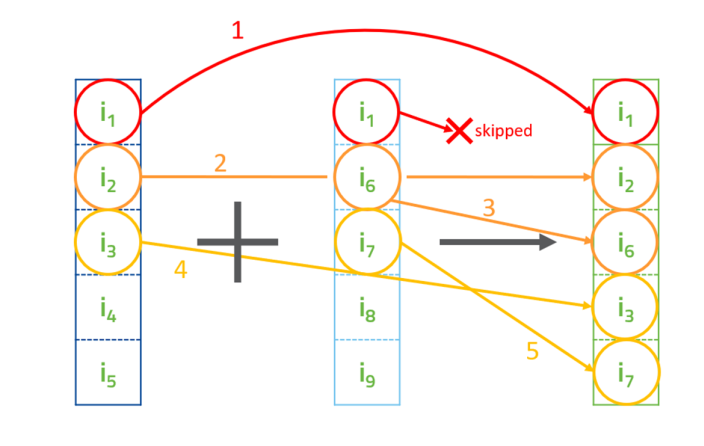
\includegraphics[width=0.35\textwidth]{imgs/072_ListCombination.png}
                \\
                \hline
                Pipelining & 
                \hfill 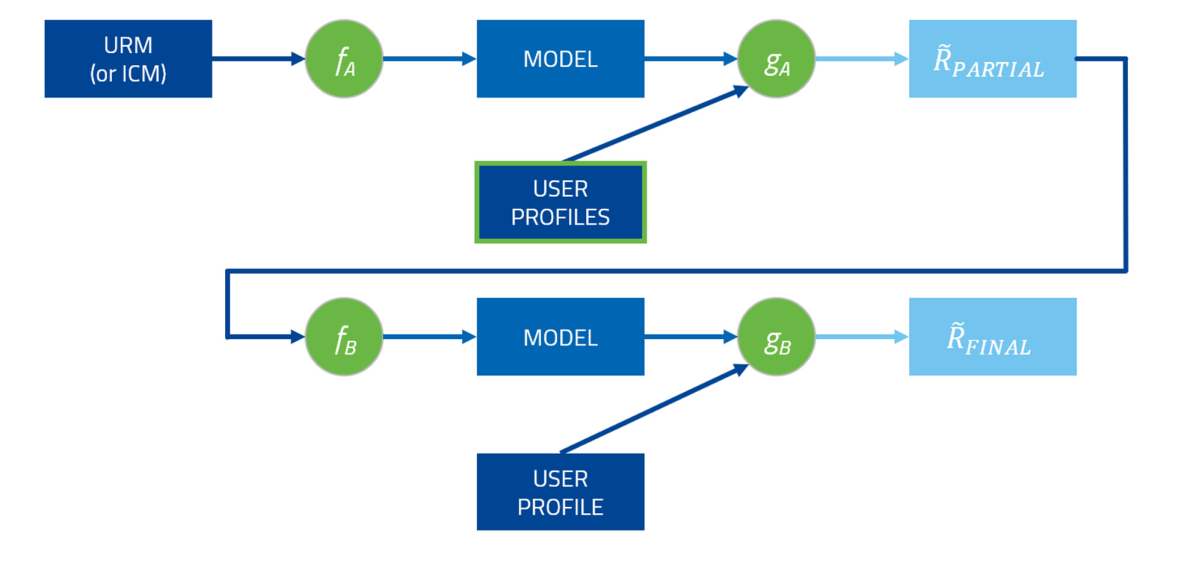
\includegraphics[width=0.35\textwidth]{imgs/073_Pipelining.png}
                \\
                \hline
                Model Merging & 
                \hfill 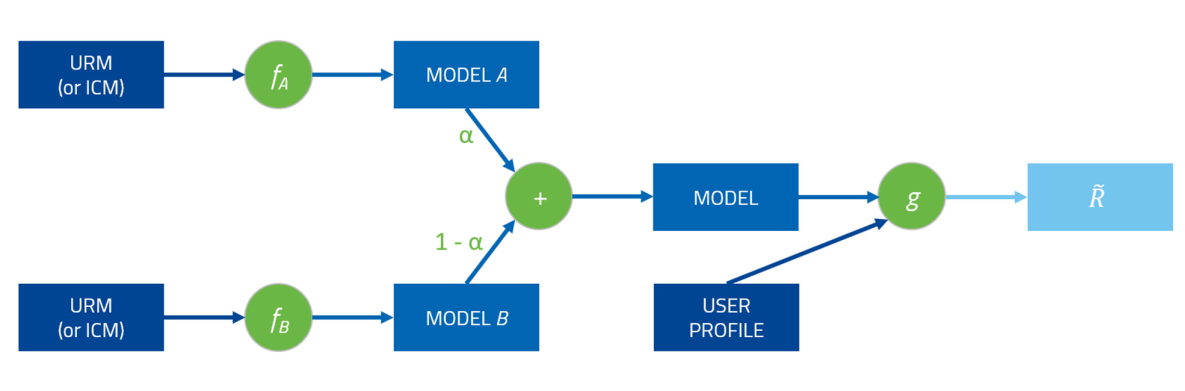
\includegraphics[width=0.35\textwidth]{imgs/074_ModelMerging.png}
                \\
                \hline
                Co-Training & 
                \hfill 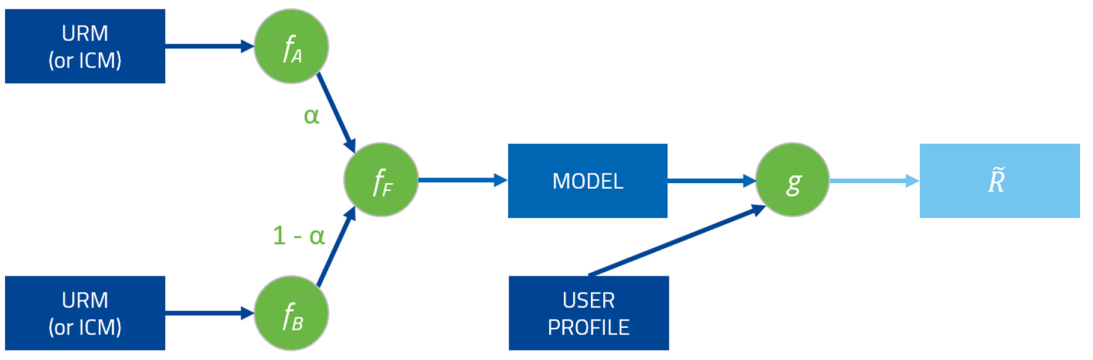
\includegraphics[width=0.35\textwidth]{imgs/075_CoTraining.png}
                \\
                \hline
                % --- SSLIM ---
                \\
                \textbf{SSLIM} (Co-Training Technique)&  
                \\
                Optimization &
                $
                    S^* = \min_S \alpha ||R - RS ||^2_F + (1 - \alpha) ||F - SF ||^2_F
                $
                \\
                Rating Prediction &
                $
                    \hat{r}_{ui} = \frac{\sum_j s_{ji} r_{uj}}{\sum_j s_{ji}}
                $
                \\
                Feature Prediction &
                $
                    \hat{f}_{ik} = \sum_j s_{ij} f_{jk}
                $
            \end{tabular}
        \end{minipage}
    };

\node[fancytitle, right=10pt] at (box.north west) {Hybrid Recommenders};
\end{tikzpicture}




%% ---- 8. Graph-Based Recommenders ----
\begin{tikzpicture}
    \node [mybox] (box) {
        \begin{minipage}{0.48\textwidth}
            \begin{tabular}{lp{0.5\textwidth}}
                \textbf{Random Walk Probability} & 
                $p_{ij} = \frac{g_{ij}}{\sum_j g_{ij}}$
                
                $
                    d_i = \sum_j g_{ij}
                $
                \\
                \textbf{Next Step Probability} & 
                $\Pi_i^{k+1} = \sum_j \Pi_j^k \cdot p_{ji}$
                \\
                \textbf{Matrix Form} & 
                $\Pi^{k+1} = P \cdot \Pi^k$
                \\
                \textbf{Steady State} & 
                $\Pi = P \cdot \Pi$
                \\
                \textbf{Probability Constraint} & 
                $\sum \Pi_i = 1$
                \\
                \hline
                \textbf{Matrix G} &
                \hfill \includegraphics[width=0.35\textwidth]{imgs/08_MatrixG.png}
                \\
            \end{tabular}
                        
        \end{minipage}
    };
    
    \node[fancytitle, right=10pt] at (box.north west) {Graph-Based Recommenders};
\end{tikzpicture}

\vspace{1cm}

\begin{tikzpicture}
    \node [mybox] (box) {
        \begin{minipage}{0.48\textwidth}
            \begin{tabular}{lp{0.5\textwidth} l}
                \textbf{PageRank} & \\
                Random Walk and Restart & 
                $
                    \prod = \gamma \prod \cdot P + (1-\gamma) \prod_{0}
                $
                \\
                \hline
                \textbf{P3Alpha $P_3\alpha$} & \\
                Metapath & $U \rightarrow I \rightarrow U \rightarrow I$\\
                
                Probability & 
                $
                    P_{UI} = (diag(\frac{1}{d_u}) \cdot R)^\alpha
                $

                $
                    P_{IU} = (diag(\frac{1}{d_i}) \cdot R^T)^\alpha
                $
                \\
                Recommendation & 
                $
                    \prod = \gamma \prod \cdot P^3
                $

                $
                    = \gamma \prod \cdot P_{UI} \cdot P_{IU} \cdot P_{UI}
                $

                $
                    = \gamma \prod \cdot P_{UI} \cdot S
                $
                \\
                Disadvantages & Strong popularity bias 

                \\
                \hline
                \textbf{RP3Beta $RP_3\beta$} & (penalize popular items)

                \\
                Similarity & 
                $
                    S_{ij} = 
                    \frac   {1}
                            {d_j^\beta} 
                    \sum_{u \in U} 
                            (\frac{r_{ui} r_{uj}}{d_i d_j})^\alpha
                $

            \end{tabular}

            \begin{tcolorbox}[colback=gray!5, colframe=gray!80!black, title={Cosine Similarity Correlation}]
                As seen above, without the parameter $\alpha$, the random walk will end up building the same similarity matrix $S$ as the one obtained by the cosine similarity (for \textbf{implicit ratings}).
                \begin{center}
                $
                    S_{ij} = 
                    [P_{IU} \cdot P_{UI}]_{ij} 
                    = \sum_{u \in U} \frac{r_{ui} r_{uj}}{d_i d_j} 
                $
                \end{center}
            \end{tcolorbox}

                        
        \end{minipage}
    };
    
    \node[fancytitle, right=10pt] at (box.north west) {Graph-Based - 2};
\end{tikzpicture}
%% ---- 9. Deep Learning Recommenders ----
\begin{tikzpicture}
    \node [mybox] (box) {
        \begin{minipage}{0.48\textwidth}
            \begin{tabular}{lp{0.5\textwidth}}
                Binary Cross Entropy $\arg \min_{\theta} =$ & 
                \sloppy
                $
                    - \frac{1}{N} \sum^N 
                            \left[ r_{ui} \log(\tilde{p}_{ui}(\theta)) 
                            + (1 - r_{ui}) \log(\tilde{p}_{ui}(\theta)) \right]
                $
                \\
                Sampling &
                    \begin{itemize}[label={--}, topsep=0cm, parsep=0cm, itemsep=0cm]
                        \item[$\times$] Cannot use ground truth (too many negative samples)
                        \item[$\times$] Cannot use just positive samples (no learning)
                        \item[$\checkmark$] Subsample among + and - interaction with probability $p=0.5$
                    \end{itemize}
                
                \\

                % --- AUTOENCODERS ---
                \textbf{Autoencoder} & \\
                \hline
                Reconstruction Loss & MSE, BCE
                \\
                Steps & 
                \begin{itemize}[label={--}, topsep=0cm, parsep=0cm, itemsep=0cm]
                    \item Sample a user profile $r_u$
                    \item Ecode it $e_u = g_e(r_u)$
                    \item Decode it $\tilde{r}_u = g_d(e_u)$
                    \item Rank the items
                \end{itemize}
                \\
                
                % --- EaseR ---
                \textit{EaseR} & (Item-Based similarity CF model)
                \\
                \hline
                Loss Function $S^* = $ & 
                $
                    \arg \min_{S} 
                    || R - RS ||_F 
                    + \lambda || S ||_F 
                    +  2\vec{\gamma} \odot diag(S)
                $

                $
                    \vec{\gamma} \in \mathbb{R}^{|I|}
                $
                \\
                Constraints & 
                $
                    diag(S) = 0
                $
                \\
                Similarity Matrix & 
                $
                    P = (R^T \cdot R + \lambda I_{|I|})^{-1}
                $
                
                $
                    S^* = I_{|I|} - P \cdot diag( \mathbf{1} 
                            \oslash diag(P))
                $
                \\
                Pros and Cons & 
                \begin{itemize}[label={}, topsep=0cm, parsep=0cm, itemsep=0cm]
                    \item[$\checkmark$] Fast and highly efficient
                    \item[$\checkmark$] Due the Frobenius norm, it tries to compute $R = RS$, thus repoducing the input as output such as an autoencoder.
                    \item[$\times$]  Computing P is memory intensive
                \end{itemize}
                \\
            \end{tabular}
            \begin{tcolorbox}[colback=gray!5, colframe=gray!80!black, title={Autoencoders and Item-Item Similarity Correlation}]
                Given a shallow autoencoder with no hidden layers and embedding size $K$, if $f = I$ and $b_e,b_d = 0$ then:
                \begin{center}
                $
                    e_u = f_e(r_u \cdot W_e + b_e) = r_u \cdot W_e
                $

                $
                    \tilde{r}_u = f_d(e_u \cdot W_d + b_d) = e_u \cdot W_d = r_u \cdot W_e \cdot W_d
                $
                \end{center}

                Since 
                $
                    W_e \in \mathbb{R}^{|I| \times K}, W_d \in \mathbb{R}^{|K| \times |I|}
                $

                We can derive the assymmetric (or symmetric, if encoder and decoder share parameters) similarity matrix $S$ as:
                $
                    S = W_e \cdot W_d
                $
            \end{tcolorbox}
        \end{minipage}
    };


    \node[fancytitle, right=10pt] at (box.north west) {DL for RECSYS};
\end{tikzpicture}


\begin{tikzpicture}
    \node [mybox] (box) {
        \begin{minipage}{0.48\textwidth}
            \begin{tabular}{lp{0.5\textwidth}}
                 % -- denoising %
                 Denoising Autoecoders & \\
                
                 \hline
 
                 Risks &
                 \begin{itemize}[label={}, topsep=0cm, parsep=0cm, itemsep=0cm]
                     \item[$\times$]  The encoder might create a poor embedding for new user profiles
                     \item[$\times$]  The decoder could lack on reconstruct correctly portion of the embedding space
                 \end{itemize}
                 \\
                 Denoising Salt \& Pepper &
                 \begin{itemize}[label={--}, topsep=0cm, parsep=0cm, itemsep=0cm]
                     \item Dropout, remove a number of positive interactions
                     \item Random add a number of positive interactions
                 \end{itemize}
                 \\

                 % --- Variational Autoencoders ---
                 Variational Autoencoders (Mult-VAE) & Encoding a input as a distribution
                 \\
                 \hline
                 Idea & 
                 \begin{itemize}[label={}, topsep=0cm, parsep=0cm, itemsep=0cm]
                     \item Encoder: encode the input as $\vec{\mu}, \vec{\sigma} $ of a Gaussian
                     \item Decoder: sample from the Gaussian and decode it $\vec{e} \tilde N(\vec{\mu}, \vec{\sigma})$
                     \item Learn the probability distribution $P(\theta | z)$.
                     
                 \end{itemize}
                 \\
                 Reparametrization Trick & 
                 $
                     \vec{e} = \vec{\mu} + \vec{\sigma} \odot \vec{\epsilon}
                 $
                 Where
                 $
                    \vec{\epsilon} \sim \mathcal{N}(0, 1)
                 $
                 \\
                 % --- TWO TOWER MODELS ---
                 \textbf{Two Tower Models} & \\
                 \hline
                  

                 &
                 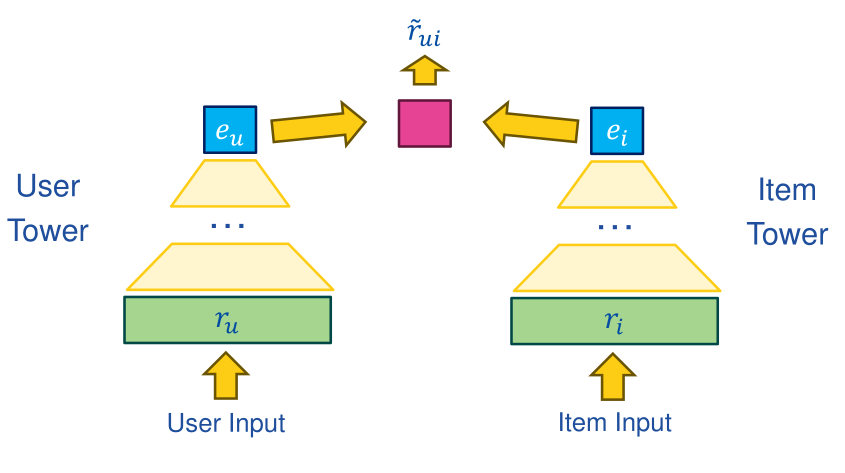
\includegraphics[width=0.35\textwidth]{imgs/090_TwoTowerModel.png}
                 \\
                 Pros and Cons &                 
                 \begin{itemize}[label={--}, topsep=0cm, parsep=0cm, itemsep=0cm]
                     \item[$\checkmark$] Can use any loss function (it does not have to reconstruct the input)
                     \item[$\checkmark$] User and item input can be of different types
                     \item[$\times$] Need to compute several ranking predictions $\tilde{r}_{ui}$
                     \item[$\times$] If the input is a one-hot encoding, it is \textbf{memory based}
                 \end{itemize}
             \end{tabular}
            \begin{tcolorbox}[colback=gray!5, colframe=gray!80!black, title={Two tower models as Matrix Factorization}]
                Consider a two-tower model with no hidden layers, embedding size $K$ and both
                user and item input one-hot encoded $x_u$ , $x_i$. If $f = I$ and $b_u, b_i, I = 0$:
                    
                $\tilde{r}_{ui} =  W_u^U \cdot W_i^I$
                Where
                $
                    W_u^U \in \mathbb{R}^{|U| \times K}, W_i^I \in \mathbb{R}^{|I| \times K}
                $
                Then we have a Matrix Factorization model with $K$ latent factors, $X = W_u^U$ and $Y = W_i^I$
            
            \end{tcolorbox}
                
        \end{minipage}
    };

\node[fancytitle, right=10pt] at (box.north west) {DL for RECSYS - 2};
\end{tikzpicture}
%% ---- 10. Graph CNN ----
\begin{tikzpicture}
    \node [mybox] (box){
        \begin{minipage}{0.48\textwidth}
        \begin{tabular}{lp{0.70\textwidth} }
            \textbf{Training} & \\
            \hline
            &
            Initialize user and item embeddings $ E^{(0)} $
            \begin{enumerate}[label={--}, topsep=0cm, parsep=0cm, itemsep=0cm]
                \item Sample a data point (depends on loss function)
                \item Apply $h$ hops of graph convolution on the nodes $E^{(h)}$
                \item Using $E^{(h)}$ compute the prediction and gradients
                \item Repeat!
            \end{enumerate}
            learn is $ E^{(0)} $
            predict is $ E^{(h)} $.
            The “message” is the node embedding.
            \\
            \textbf{LightGCN} & \\
            \hline
            &
            - weighted mean as aggregation function

            - Loss function is BPR
            
            - Does not include self-connections
      
            \\
            &
            $
                E_u^{(h)} = \sum_{i:u,i \in R^+} \frac{1}{\sqrt{d_u \cdot d_i}}\cdot E_i^{(h-1)}
            $

            $
                E_i^{(h)} = \sum_{u:u,i \in R^+} \frac{1}{\sqrt{d_u \cdot d_i}}\cdot E_u^{(h-1)}
            $ 
            \\
            &
            normalized adjacency matrix $\hat{G}$:

            $
                \hat{g}_{xy}= \frac{g_{xy}}{\sqrt{d_x d_y}}
            $
            \\
            \textbf{Training} & LightGCN\\
            \hline
            &
            Initialize the embeddings $ E^{(0)} $
            \begin{enumerate}[topsep=0cm, parsep=0cm, itemsep=0cm]
                \item Apply $h$ convolution steps $E^{(h)} = \hat{G}^h \cdot E^{(0)}$
                \item Draw a BPR sample $u,i,j$ such that $u,i \in R^+$ and $u,j \in R^-$
                \item Compute prediction $\tilde{r}_{ui} =  E_u^{(h)} \cdot  E_i^{(h)}$ and $\tilde{r}_{uj}$
                \item Apply gradient of BPR
            \end{enumerate}
            \\

            Pros and Cons & 
            \begin{itemize}[label={}, topsep=0cm, parsep=0cm, itemsep=0cm]
                \item[$\checkmark$] Can work on different types of graphs
                \item[$\checkmark$] Can accommodate different aggregationfunctions that may have parameters themselves
                \item[$\checkmark$] Can accommodate different lossfunctions
                \item[$\times$] Have enormous computational cost
                \item[$\times$] Can exhibit high popularity bias
            \end{itemize}
            \\

            \textbf{Popularity Bias} & \\
            \hline
            
            $\hat{G}$ with SVD
            &
            \begin{center}
            $
                E^{(h)} = \hat{G} ^h \cdot E^{(0)} 
            $    

            $
                = (V \cdot \Sigma \cdot V^T )^h \cdot E^{(0)} 
            $

            $    
                = V \cdot \Sigma^h \cdot V^T \cdot E^{(0)}
            $
            \end{center}
            \\
            &
            - Large singular values, strongly popularity-based

            - Small singular values, fine-grained signals
            \\
            \textbf{Filter Function} & \\
            \hline  
            
            $f$ modifies $\Sigma$ 
            &
            $
                E^{(h)} = \hat{G} ^h \cdot E^{(0)} = V \cdot f(\Sigma)^h \cdot V^T \cdot E^{(0)}
            $
            \\
        \end{tabular}
    \end{minipage}
};

 \node[fancytitle, right=10pt] at (box.north west) {Graph Convolutional Networks};  
\end{tikzpicture}



\begin{tikzpicture}
    \node [mybox] (box){
        \begin{minipage}{0.48\textwidth}
            \begin{tabular}{lp{0.70\textwidth} }
                \textbf{GF-CF} & \\
                \hline
                &
                - Observation:small singular values disappear
               
                - Idea: use truncated SVD to compute the similarity.
                \\
        
            Normalize & 
            $
            \tilde{r}_{ui} = \frac{r_{ui}}{\sqrt{d_u d_i}}
            $ \\
            Compute item-item S: & 
            $
                S =\hat{R}^T \cdot  \hat{R} + \alpha D_I ^{-\frac{1}{2}} \cdot V_k \cdot V_k^T \cdot D_I ^{+\frac{1}{2}}
            $ \\

            Pros and Cons & 
            \begin{itemize}[label={}, topsep=0cm, parsep=0cm, itemsep=0cm]
                \item[$\checkmark$] Fast computation of the similarity and very effective
                \item[$\checkmark$] Flexible, change the exponent of the degree matrix
                \item[$\times$] The similarity is dense (high memory requirement, slow prediction)
                \item[$\times$] Applying KNN is difficult, large \# of neighbors
            \end{itemize}
        \end{tabular}
    \end{minipage}
};

\node[fancytitle, right=10pt] at (box.north west) {Graph-Filter Collaborative Filtering};  
\end{tikzpicture}
%% ---- 11. Factorization Machines ----
\begin{tikzpicture}
    \node [mybox] (box){
        \begin{minipage}{0.48\textwidth}
            \begin{tabular}{lp{0.8\textwidth}}
                Input Data &
                $
                    \begin{matrix} 
                        \text{user} & \text{item} & \text{rating} \\
                        1, 0, 0 & 1, 0, 0 & 3 \\
                        0, 1, 0 & 0, 1, 0 & 1 \\
                        \vdots & \vdots & \vdots \\
                        0, 0, 1 & 0, 0, 1 & 2 
                    \end{matrix}
                $ One hot encoding.
                
                \\
                Rating Estimation  &
                $
                    \tilde{r}^{(k)} = \omega_0 
                                    + \sum_{i=1}^n \omega_i x_i^{(k)}
                                    + \sum_{i=1}^n \sum_{j=i + 1}^n \omega_{ij} x_i^{(k)} x_j^{(k)}
                $

                \\
                Vector Form &
                $
                    \tilde{r}^{(k)} = \omega_0 + \vec{\omega} \cdot \vec{x}^{(k)} + \vec{x}^{(k)T} \cdot W \cdot \vec{x}^{(k)}
                $
                
                \\
                Loss Function &
                $
                    \arg \min_{\vec{\omega}} E(\omega) = \arg \min_{\vec{\omega}} || r^{(k)} - \tilde{r}^{(k)} ||
                $

                \\

                $W$ factorization &

                $
                    \omega_{ij} = \vec{v}_i \cdot \vec{v}_j 
                                = \sum_{h=0}^f v_{i,h} v_{j,h}
                $
                $
                    f << n \  \text{latent factors}
                $

                \\
                N parameters &
                $
                    \begin{cases}
                        1 + n + \frac{n^2 - n}{2} & \text{if not factorized} \\
                        1 + n + nf & \text{if factorized} 
                    \end{cases}
                $
                
                \\
                Imbalance Problem &
                \begin{itemize}[label={}, topsep=0cm, parsep=0cm, itemsep=0cm]
                    \item[$\times$] If ratings are implicit, lead to predict only $1$s
                    \item [$\checkmark$] Random select non rated items for every user
                    \item [$\checkmark$] Use the same number of positive and negative samples
                \end{itemize}
                \\
            \end{tabular}

            \begin{tcolorbox}[colback=gray!5, colframe=gray!80!black, title={Factorization Machines as SVD++}]
                Using only collaborative data, the factorization machine is equivalent to SVD++, since one-hot encoding we can rewrite the factorization machine as:
                \\
                \begin{equation}
                    \tilde{r}^{(k)} = \omega_0 + \omega_i 
                                    + \omega_u +
                                    V_i \cdot V_u^T  
                \end{equation}
                \\
                Equivalent to SVD++.

                We need to add \textbf{Context} data, for example from a ICM model.
            \end{tcolorbox}
        \end{minipage}
    };


\node[fancytitle, right=10pt] at (box.north west) {Factorization Machines};
\end{tikzpicture}
\end{multicols*}
\end{document}